\documentclass{beamer}
\usepackage[spanish]{babel}
\usepackage{beamerthemeshadow}
\usepackage{pgf}
\usepackage{eurosym}
\usepackage{array}% http://ctan.org/pkg/array
\usepackage{fontspec}
\usepackage{fontawesome}
\newcolumntype{M}{>{\centering\arraybackslash}m{\dimexpr.25\linewidth-2\tabcolsep}}
\usepackage{hyperref}
\hypersetup{
  breaklinks=true,
  urlcolor=blue,
}

\usetheme{CambridgeUS}
\usefonttheme{structurebold}

\setbeamertemplate{itemize item}[triangle]

\begin{document}


\title{Sistemas de control de versiones distribuidos}
\subtitle{Controla las versiones de tu trabajo con GIT}
\author[Nacho Álvarez]{\texorpdfstring{Nacho Álvarez
  \\ \faTwitter \hspace{5pt}@neonigmacdb
  \\ \faEnvelope \hspace{5pt}neonigma@gmail.com}{Author}}

\institute[WUL4]{
\includegraphics[height=0.6cm]{imgs/wul4.png}}
\date{\today}



\frame{\centering 
\includegraphics[height=1cm]{imgs/training-thursday.png} \titlepage}

\section[Índice]{}
\frame{\tableofcontents}


\section{Acerca de mí}
\frame
{
\frametitle{Who?}
\begin{itemize}
\item \textbf{Trayectoria profesional:} soporte UCO, desarrollador Web, desarrollador / integrador distribuciones GNU/Linux.
\item \textbf{Actualmente:} WUL4 Córdoba (mobile + backend developer)
\item \textbf{Involucrado en:}
\begin{center}
  $\vcenter{\hbox{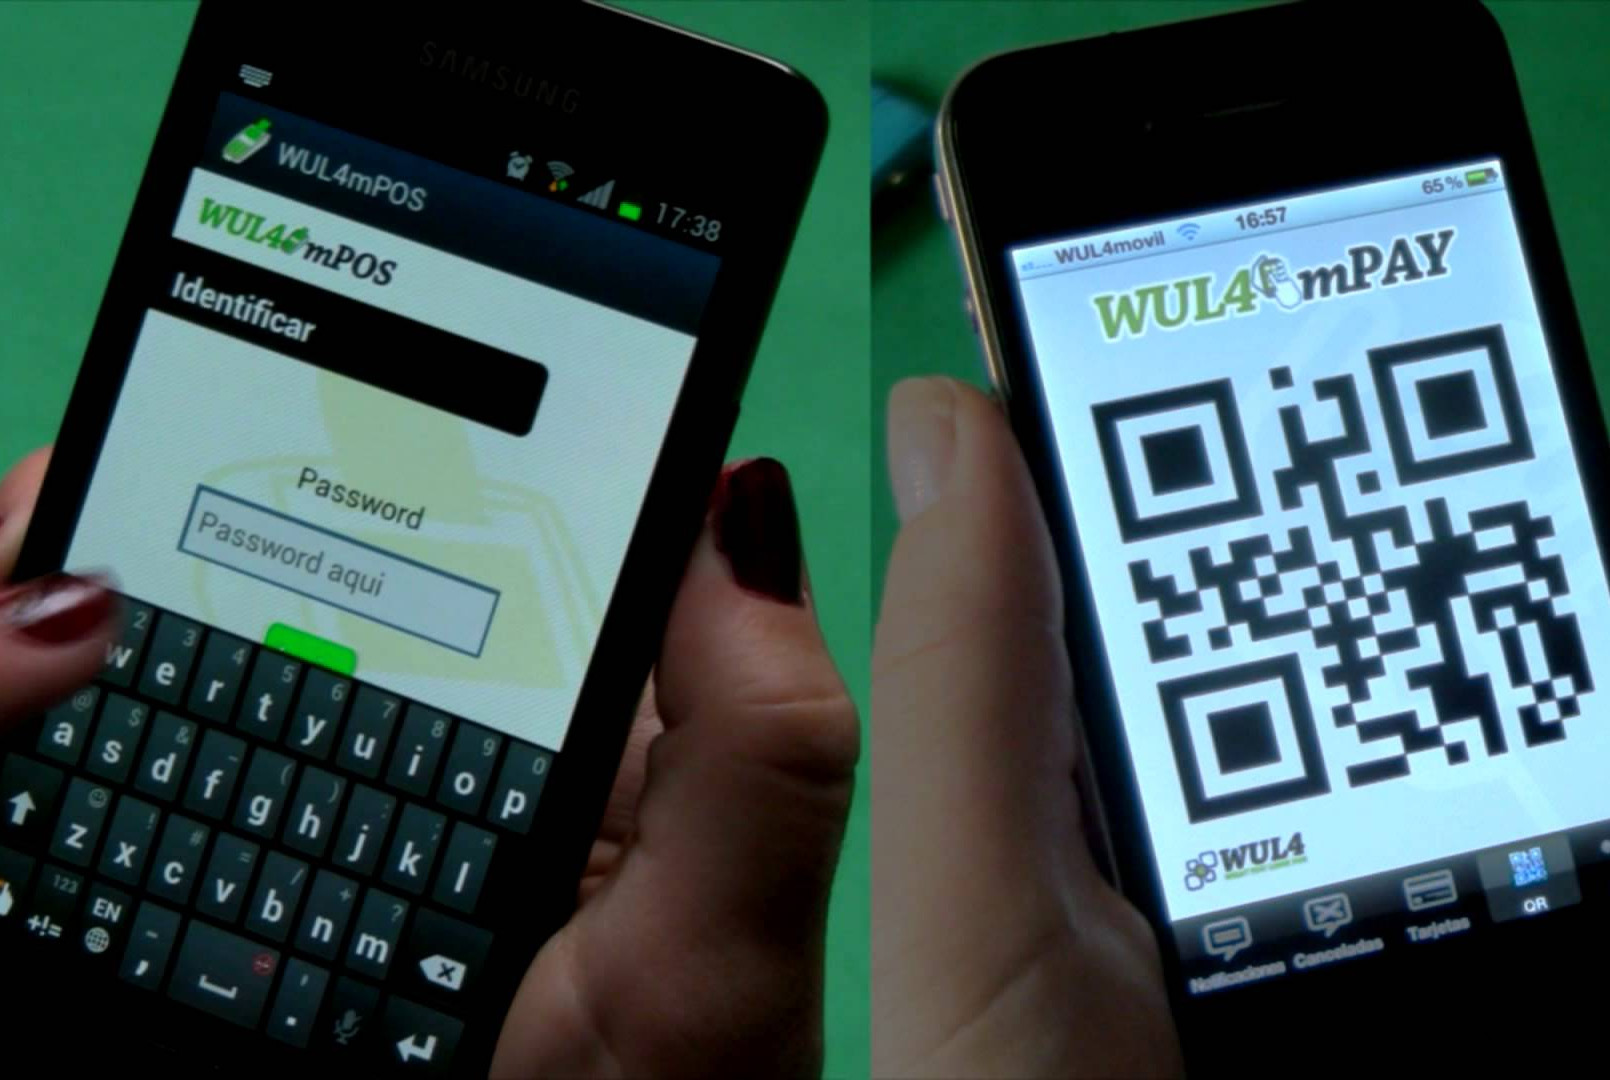
\includegraphics[height=1.25in,width=1.5in]{imgs/wul4mpay.jpg}}}$
  $\vcenter{\hbox{
\includegraphics[height=1.25in]{imgs/wul4bus.jpg}}}$
  $\vcenter{\hbox{
\includegraphics[height=1.25in]{imgs/id.jpg}}}$
  $\vcenter{\hbox{
\includegraphics[width=0.9in]{imgs/redsys.jpg}}}$
\end{center}
\end{itemize}
}

\section{Definiciones}
\frame
{
\frametitle{Definiciones}
\begin{itemize}
\item \textbf{Control de versiones:} gestión de los diversos cambios que se realizan sobre los elementos de algún producto
\item Una \textbf{versión}, \textbf{revisión} o \textbf{edición} de un producto, es el \textbf{estado} en el que se encuentra dicho producto en un \textbf{momento} dado de su desarrollo o modificación
\item Los \textbf{sistemas} de control de versiones (SCV) vienen a automatizar parcialmente la gestión de este control de cambios
\item Existen SCV \textbf{centralizados} (repositorio único remoto) y SCV \textbf{distribuidos} (cada usuario su repositorio local + remoto)
\item Los más famosos y de más trayectoria son: SVN, GIT, Mercurial, Bazaar, ClearCase, Perforce...
\end{itemize}
}

\section*{SCV centralizados}
\frame
{
\frametitle{Ventajas SCV centralizados}
\begin{itemize}
\item En los sistemas distribuidos hay un \textbf{mayor bloqueo} del estado final del proyecto que en los sistemas centralizados.
\item En los sistemas centralizados las versiones vienen identificadas por un \textbf{número de versión}. En lugar de eso, en los sistemas distribuidos, cada versión tiene un identificador (hash) al que se le puede asociar una etiqueta (tag).
\item La \textbf{curva de aprendizaje} es sensiblemente menor que en los sistemas distribuidos
\item Requiere \textbf{menor intervención} del mantenedor
\end{itemize}
}

\section*{SCV distribuidos}
\frame
{
\frametitle{Ventajas SCV distribuidos}
\begin{itemize}
\item Necesita \textbf{menos operaciones en red} => mayor autonomía y una mayor rapidez.
\item Aunque se \textbf{caiga} el \textbf{repositorio remoto} la gente puede seguir trabajando
\item Alta probabilidad de \textbf{reconstrucción} en caso de falla debido a su arquitectura distribuida
\item Permite mantener \textbf{repositorios centrales más limpios}, el mantenedor decide
\item El \textbf{servidor remoto} requiere \textbf{menos recursos} que los que necesitaría un servidor centralizado ya que gran parte del trabajo lo realizan los \textbf{repositorios locales}.
\item Al ser los sistemas distribuidos \textbf{más recientes} que los sistemas centralizados, y al tener \textbf{más flexibilidad} por tener un repositorio local y otro/s remotos, estos sistemas han sido diseñados para hacer fácil el uso de \textbf{ramas locales y remotas} (creación, evolución y fusión) y poder aprovechar al máximo su potencial. 
\end{itemize}
}

\section{¿Por qué GIT?}
\usebackgroundtemplate{%
  
\includegraphics[width=\paperwidth,height=\paperheight]{imgs/git-no.jpg}} 
\frame
{
\frametitle{¿Por qué GIT?}
}

\usebackgroundtemplate{%
  
\includegraphics[width=\paperwidth,height=\paperheight]{imgs/git-si.jpg}} 
\frame
{
\frametitle{¿Por qué GIT?}
}
\usebackgroundtemplate{}
\frame
{
\frametitle{En números}

\includegraphics[height=1cm]{imgs/git-bitbucket.png}
\begin{itemize}
 \item Enfocado a \textbf{código privado} (Facebook, Cisco, Adobe, Opera...)
 \item Más de \textbf{1 millón} de usuarios registrados
 \item Integración del resto del ecosistema software: Bamboo (CI), Confluence (Doc), Jira (project tracking), SourceTree (GUI)...
 \item Se cobra por \textbf{número de integrantes de equipo}: 0-5 (gratis), 6-10 (\$10 month), 11-25 (\$25 month), 26-50 (\$50 month)...
\end{itemize}


\includegraphics[height=1cm]{imgs/git-github.png}
\begin{itemize}
 \item Enfocado a \textbf{código abierto} (bootstrap, nodejs, jquery...)
 \item Más de \textbf{4 millones} de usuarios registrados y \textbf{8 millones} de \textbf{repositorios} creados
 \item Se cobra por \textbf{repositorios privados}: 5 (\$7 month), 10 (\$12 month), 20 (\$22 month), 50 (\$50 month)
\end{itemize}
}

\section{Arquitectura SCV}
\frame
{
\frametitle{Arquitectura SCV centralizado}
\begin{itemize}
 \item Todo el mundo actualiza un mismo repositorio central remoto
\end{itemize}

\begin{center}
 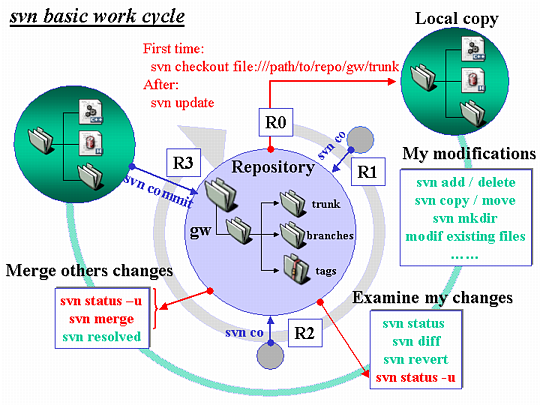
\includegraphics[height=5cm]{imgs/svnscheme.png}
\end{center}
}

\frame
{
\frametitle{Arquitectura SCV distribuido}
\begin{itemize}
 \item Todo el mundo mantiene su copia del proyecto
 \item Cada integrante del equipo trabaja en sus propias funcionalidades en su repositorio local particular
 \item El mantenedor del repositorio acepta o no las modificaciones de los integrantes
\end{itemize}

\begin{center}
 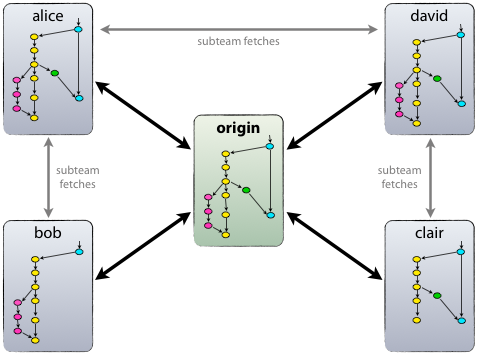
\includegraphics[height=5cm]{imgs/gitscheme.png}
\end{center}
}

\frame
{
\frametitle{GIT}
\begin{itemize}
 \item Nacido de la mente de Linus Torvalds. Versión 1.0 en 2005. 
\end{itemize}

\begin{center}
  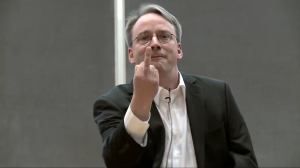
\includegraphics[height=2cm]{imgs/linus.png}    
\end{center}

\begin{itemize}
 \item Se buscaba una manera de gestionar la ingente cantidad de código del kernel de Linux
 \item Toma el diseño de versiones anteriores de BitKeeper y Monotone
 \item Git se basa en \textit{snapshots}, cada commit es una copia completa del código comprimida en binario, lo que le imprime velocidad. Usan compresión delta zlib para optimizar el espacio.
 \item Se ha medido git log frente a svn log, git opera 100x más rápido
 \item Se opera siempre en local (de ahí el incremento de velocidad) y cuando se tienen listos los cambios se suben a remoto
\end{itemize}
}
\section{Flujo de trabajo en GIT}
\frame
{
\frametitle{Flujo de trabajo en GIT}
\begin{center}
 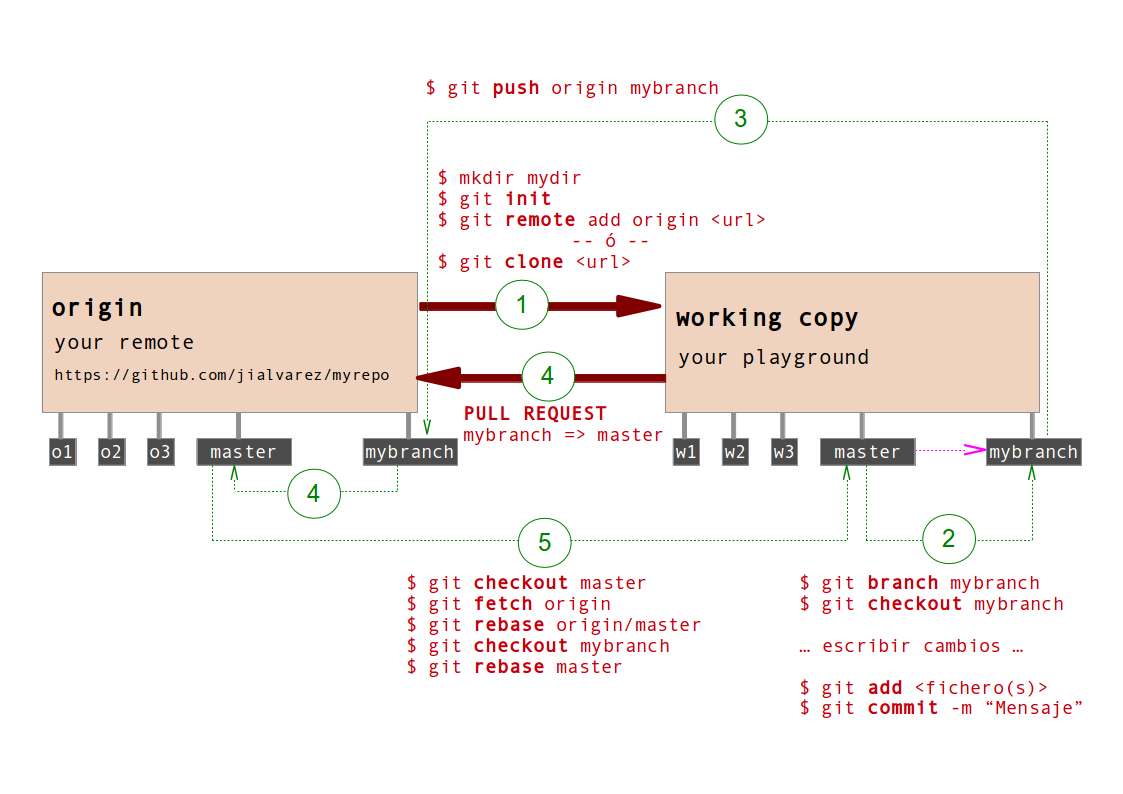
\includegraphics[height=7cm]{imgs/gitworkflow.png}
\end{center}
}

\frame
{
\frametitle{Etapas de un fichero (I)}
\begin{framed}
\# \textbf{Archivos sin seguimiento:}\\
\#   (use git add <archivo>... para incluir lo que se ha de ejecutar)\\
\#\\
\#	\textcolor{red}{fichero.tex}
\end{framed}

\begin{itemize}
 \item Son archivos que aún no forman parte del repositorio local ni del remoto
 \item Al añadirlos pasan a la etapa III
\end{itemize}
}

\frame
{
\frametitle{Etapas de un fichero (II)}
\begin{framed}
\# \textbf{Cambios no preparados para el commit:}\\
\#   (use git add <archivo>... para actualizar lo que se ejecutará)\\
\#   (use git checkout -{}- <archivo>... para descartar cambios en el directorio de trabajo)\\
\#\\
\#	\textcolor{red}{modificado:   advanced.tex}\\
\#	\textcolor{red}{modificado:   principal.pdf}\\
\end{framed}

\begin{itemize}
 \item Son ficheros ya añadidos previamente pero que aún no han sido \textit{marcados} para comitear
 \item Al añadirlos pasan a la etapa III
 \item Si le aplicamos un \textit{checkout} vuelven a la etapa I
\end{itemize}
}

\frame
{
\frametitle{Etapas de un fichero (III)}
\begin{framed}
\# \textbf{Cambios para hacer commit:}\\
\#   (use git reset HEAD <archivo>...para eliminar stage)\\
\#\\
\#	\textcolor{green}{modificado:   workflow.tex}\\
\end{framed}

\begin{itemize}
 \item Son ficheros ya añadidos previamente y marcados para comitear
 \item Si le aplicamos un \textit{reset HEAD} vuelven a la etapa II
 \item En esta etapa es donde se puede \textit{\textbf{comitear}} y hacer \textit{\textbf{push}}
\end{itemize}
}

\frame
{
\frametitle{Git branching}

\begin{tabular}[t]{m{5cm}m{6cm}}
   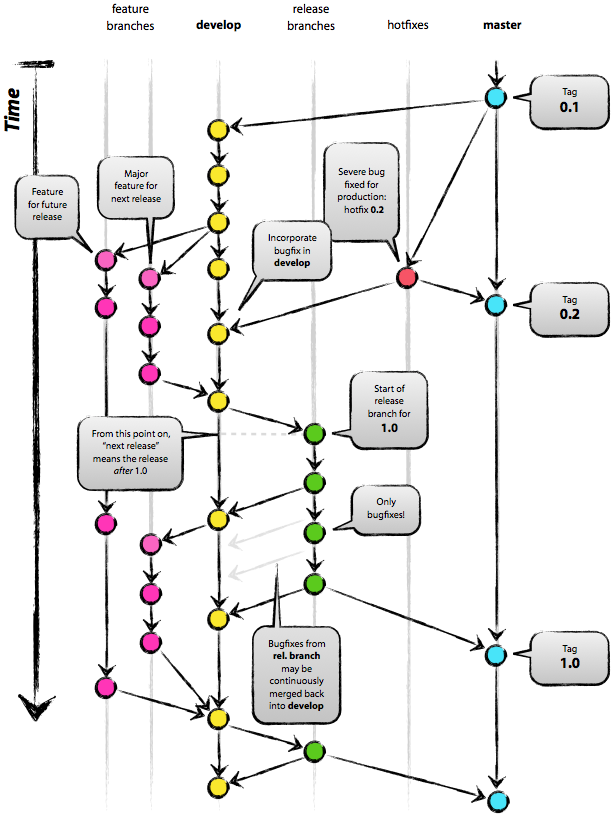
\includegraphics[height=8cm]{imgs/gitbranching.png} 
   &
   \begin{itemize}
    \addtolength{\itemindent}{0.4cm}
    \item Reglas propuestas por Vincent Driessen
    \item Ramas \textbf{master} (commits producción) y \textbf{develop} (siguiente versión planificada)
    \item Ramas \textbf{feature} (funcionalidad concreta). Se originan a partir de \textbf{develop} y vuelven a \textbf{develop}
    \item Ramas \textbf{release} (siguiente versión en producción). Se originan de \textbf{develop} y pasan a master o \textbf{develop}.
    \item Ramas \textbf{hotfix} (bugs en producción). Se originan a partir de \textbf{master} y vuelven a \textbf{master} o \textbf{develop}.
   \end{itemize}
\end{tabular}
}
\section{Demo}
\frame
{
\frametitle{Demo}
\begin{center}
 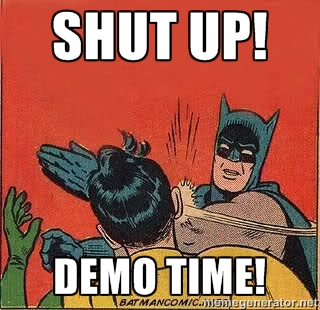
\includegraphics[height=4cm]{imgs/demo-time.jpg}
\end{center}

\begin{itemize}
 \item Crearemos nuestro propio repositorio Git en Bitbucket
 \item Crearemos nuestra rama de trabajo y subiremos cambios
 \item Propondremos la integración de estos cambios haciendo \textit{pull request}
 \item Simularemos la descarga del repositorio por parte de un compañero y subiremos nuevos cambios
 \item Actualizaremos el repo haciendo \textit{rebase} y subiremos más cambios
 \item Mostraremos cómo funciona el \textit{rebase} de manera gráfica
\end{itemize}
}

\section{Gestión de conflictos}
\frame
{
\frametitle{Merges en caso de conflicto}
\$ git \textbf{checkout} master\\
Switched to branch 'master'\\
\$ git \textbf{merge} -{}-no-ff -m 'Merged pull request \#7' mybranch \\

\begin{center}
 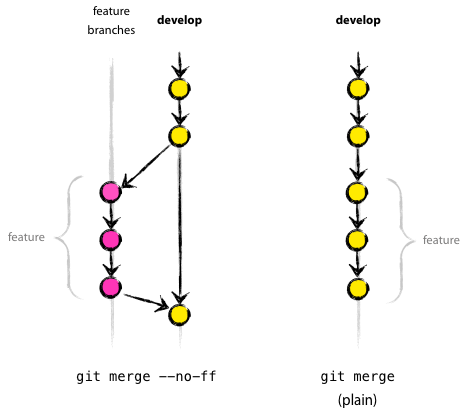
\includegraphics[height=6cm]{imgs/gitmerge.png}
\end{center}
}

\section{Más funcionalidades útiles}
\frame
{
\frametitle{Más funcionalidades útiles}
\begin{center}
 
\includegraphics[height=7cm]{imgs/koala.jpg} 
\end{center}
}

\frame
{
\frametitle{pull}
Utilizándolo sin ningún parámetro adicional -\textbf{git pull origin master}- funciona igual que un \textit{update} en Subversion. Es decir, se trae los cambios y hace \textit{merge}. Si le pasamos el parámetro \textit{-{}-rebase}, funciona como un \textit{rebase}.

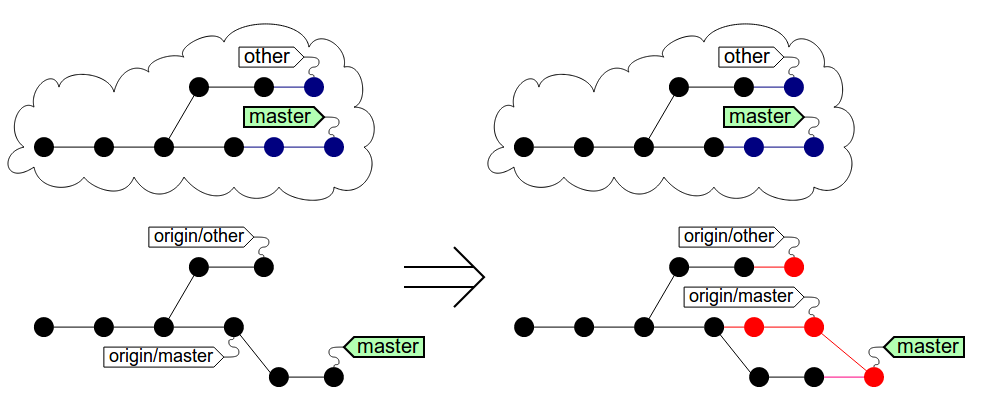
\includegraphics[height=5cm]{imgs/pull.png} 
}

\begin{frame}[fragile]
\frametitle{ignore}
El fichero \textit{.gitignore} se suele colocar en la raíz del proyecto y el contenido suele ser un listado de elementos que no queremos que sean reconocidos como ficheros del repositorio.
\footnotesize
\begin{verbatim}
neonigma@hyperion:~/things/taller-git$ cat .gitignore 
*.aux
*.bbl
*.log
*.backup
*.toc
*.dvi
*.out
neonigma@hyperion:~/things/taller-git$ git log principal.aux
neonigma@hyperion:~/things/taller-git$ 
\end{verbatim}
\end{frame}

\begin{frame}[fragile]
\frametitle{update-index}
El comando \textbf{update-index} -{}-assume-unchanged se utiliza para ficheros que accidentalmente se han \textit{comiteado} (y probablemente \textit{pusheado}) y no queremos tener en cuenta los cambios producidos en estos ficheros, ya que lo veremos como modificados en la etapa II (listo para \textit{comitear}).
\footnotesize
\begin{verbatim}
$ echo "Nueva linea\n" >> bibliografia.bib

$ git status
# En la rama master
# Cambios no preparados para el commit:
#   (use «git add <archivo>...» para actualizar lo que se ejecutará)
#   (use «git checkout -- <archivo>...« para descartar cambios en le directorio de trabajo)
#
#	modificado:   bibliografia.bib
#

$ git update-index --assume-unchanged bibliografia.bib

$ git status
# En la rama master
nothing to commit, working directory clean
\end{verbatim}
\end{frame}

\frame
{
\frametitle{revert}
  Este comando deshace un único commit aplicando el parche con la diferencia como un nuevo commit. Ejemplo: git \textbf{revert} HEAD
 \begin{tabular}{p{4cm}|p{4cm}}\\
    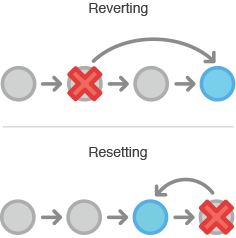
\includegraphics[height=4cm]{imgs/revert-vs-reset.png}&
    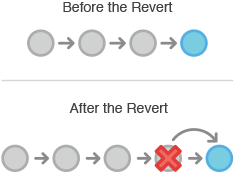
\includegraphics[height=3.5cm]{imgs/revert-sample.png}\\
 \end{tabular}

 Este comando no destruye la historia ni diverge las ramas \textit{master}. Ejemplo pack commits: git \textbf{revert} master\textasciitilde2..master
}

\frame
{
\frametitle{soft reset}
 El comando git reset -{}-soft <hash> mueve el puntero de la cabeza al hash del commit que le indiquemos.\\
 \begin{center}
    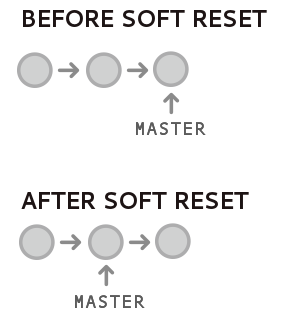
\includegraphics[height=4cm]{imgs/soft-reset.png}
 \end{center}
}

\frame
{
\frametitle{hard reset}
 El comando git reset -{}-hard <hash> mueve el puntero de la cabeza al hash del commit que le indiquemos y \textbf{destruye} toda la historia hasta dicho hash.\\
 \begin{center}
    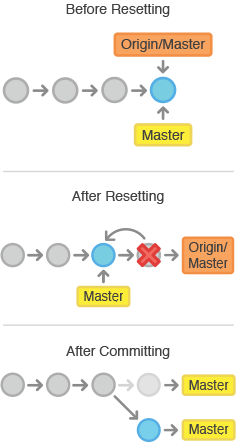
\includegraphics[height=6cm]{imgs/reset-hard.png}
 \end{center}
}

\section{Algo más avanzado}
\frame
{
\frametitle{Algo más avanzado}
\begin{center}
  
\includegraphics[height=7.5cm]{imgs/noidea.jpg}
\end{center}
}

\frame
{
\frametitle{stash}
 Se utiliza para \textit{aparcar} temporalmente los cambios actuales antes de ser comiteados. El comando se escribe únicamente git \textbf{stash}.
 \begin{framed}
 \$ git \textbf{stash} list\\
 stash@\{0\}: WIP on master: 049d078 added the index file\\
 stash@\{1\}: WIP on master: c264051... Revert added file\_size\\
 stash@\{2\}: WIP on master: 21d80a5... added number to log
 \end{framed}
 
 Recuperamos los cambios con el comando git \textbf{stash} apply <id>
}

\frame
{
\frametitle{format-patch}
 Se utiliza para generar parches que se entregarán a mantenedores de repositorios que no aceptan \textit{pull requests}.\\ \vspace{0.2cm}
 Un parche se genera con el comando git \textbf{format-patch} -{}-stdout \textit{<hash o rango de hashes>}. Esto genera tantos ficheros con parches como commits se hayan introducido como parámetro.\\ \vspace{0.2cm}
 Para aplicar los parches, se utiliza el comando git \textbf{am} -{}-signoff < \textit{file.patch}
}

\frame
{
\frametitle{squash}
 Se utiliza dentro de lo que se llama el \textit{rebase interactivo}, para unir varios commits en uno solo antes de entregarlos al repositorio remoto. El proceso sería:
 \begin{itemize}
  \item Comiteamos tantas veces como queramos: git commit -m ``mensaje''
  \item Si por ejemplo hemos hecho 2 commits, ejecutamos el rebase interactivo con: git \textbf{rebase} -i HEAD\textasciitilde2\\ \vspace{0.2cm}
  \footnotesize
   pick 4ca2acc commit file1\\
   pick 7b36971 commit file2\\
   
   \# rebase 41a72e6..7b36971 onto 41a72e6\\
   \#\\
   \# commands:\\
   \#  p, pick = use commit\\
   \#  r, reword = use commit, but edit the commit message\\
   \#  e, edit = use commit, but stop for amending\\
   \#  s, squash = use commit, but meld into previous commit\\
   \#  f, fixup = like ``squash'', but discard this commit's log message\\
   \#  x, exec = run command (the rest of the line) using shell
\end{itemize}
}

\frame
{
\frametitle{cherry-pick}
 \begin{itemize}
  \item Permite incorporar commits individuales a tu rama de trabajo
  \item El commit procederá de otra rama cualquiera
  \item La sintaxis: git \textbf{cherry-pick} <hash\_commit>
  \item La ventaja de esto es aprovechar funcionalidades comiteadas por otros miembros del equipo
  \item Si la recuperación del commit trae problemas de mezclado, se puede abortar esta recuperación con git \textbf{cherry-pick} -{}-abort
 \end{itemize}
}

\frame
{
\frametitle{reflog}
 \begin{itemize}
  \item Con git \textbf{log} vemos todos los commits realizados (historia)
  \item git \textbf{reflog} nos permite revisar todas las \textbf{acciones} realizadas
  \item Se puede utilizar para recuperar commits o ramas perdidas al utilizar git \textbf{reset}
  \item Los commits reseteados están disponibles durante 30 días, y los normales, durante 90 días
  \item[] \footnotesize 
	neonigma@hyperion:~/things/taller-git\$ git reflog\\
	abec02f HEAD@{0}: merge foo: Merge made by recursive.\\
	9bdbd83 HEAD@{1}: 9bdbd83: updating HEAD\\
	2d90ece HEAD@{2}: merge foo: Fast-forward\\
	9bdbd83 HEAD@{3}: checkout: moving from foo to master\\
	2d90ece HEAD@{4}: commit: hello\\
	9bdbd83 HEAD@{5}: checkout: moving from master to foo
\end{itemize}
}

\frame
{
\frametitle{submodules}
 \begin{itemize}
  \item submodules permite \textit{linkar} un repositorio dentro de otro
  \item Es una funcionalidad amada y odiada a partes iguales, por sus fuertes ventajas y desventajas
  \item Otras alternativas pasan por usar \textbf{subtree}, \textbf{gitslave} o \textbf{repo}
  \item Submodules es usado por:
    \begin{center}
      $\vcenter{\hbox{
\includegraphics[height=1.25in,width=1.5in]{imgs/gecos.png}}}$
      $\vcenter{\hbox{
\includegraphics[height=1.25in]{imgs/gnome.png}}}$
      $\vcenter{\hbox{
\includegraphics[height=1.25in]{imgs/android.png}}}$
    \end{center}
 \end{itemize}
}

\frame
{
\frametitle{submodules}
 \begin{itemize}
 \item Añadir un repositorio git como submódulo
  \begin{itemize}
    \item git \textbf{submodule} add [-b master] git@bitbucket.org:jialvarez/testproject.git
    \item git \textbf{commit} -m ``Añadimos submódulo testproject''
    \item git \textbf{push} <remote> <branch>
  \end{itemize}

 \item A partir de aquí el trabajo con el submódulo sería de manera normal, como un repositorio git cualquiera
 \item Tras actualizar el submódulo (add + commit + push), debemos actualizar también la referencia del padre de la misma manera
 \item ¡¡¡¡¡¡CUIDADO!!!!!! 
  \begin{itemize}
    \item Si hacemos \textit{push} en el proyecto padre y no en el proyecto hijo, el siguiente que haga un \textit{clone} del proyecto, no podrá descargarse todo el código al faltarle referencias
    \item Si no pusheamos el hijo y hacemos un par de commits, y luego tratamos de actualizar el padre con git submodule update, dejamos al hijo en DETACHED mode (sin ramas)
  \end{itemize}
 \end{itemize}
}

\frame
{
\frametitle{submodules}
 \begin{itemize}
 \item Descargar / actualizar repositorio conteniendo submódulos
  \begin{itemize}
   \item git \textbf{clone} git@bitbucket.org:jialvarez/testproject.git
   \item git \textbf{submodule} init
   \item git \textbf{submodule} update
  \end{itemize}

 \item Para hacer un barrido por todos los módulos y actualizarlos: \\git \textbf{submodule} foreach git pull origin master
 \item Para borrar un submódulo:
  \begin{itemize}
   \item Se eliminan sus líneas de configuración del fichero .gitmodules
   \item Se eliminan sus líneas de configuración del fichero .git/config
   \item Se ejecuta: git \textbf{rm} -{}-cached <path/to/submodule>
  \end{itemize}

  \item submodules es parte del \textit{core} de git y está disponible para todos los SO y bien integrado en GUIs
 \end{itemize}
}

\frame
{
\frametitle{lolcommits}
 \begin{itemize}
  \item Te permite tomar una foto desde la Webcam de manera automática cada vez que haces git commit
  \item Puede descargarse aquí: \url{http://mroth.github.io/lolcommits/}
  \item Tiene una lista de plugins para cambiar el vocabulario de commits, subir automáticamente las imágenes a un servidor, tuitear, etc.
  \item Se pueden hacer gif animados con las imágenes tomadas: \url{http://nacho-alvarez.es/descargas/myimage.gif}
  \item En Linux y Mac OS X es ultrasencillo de instalar, en Windows algo más complejo
  \item Para habililitar lolcommits en un repositorio git, sólo hay que escribir \textbf{lolcommits} -{}-enable
  \item Si queremos ver la última imagen: \textbf{lolcommits} -{}-last , si queremos abrir la carpeta: \textbf{lolcommits} -{}-browse
 \end{itemize}
}


\section{Enlaces de interés}
\frame
{
\frametitle{Enlaces de interés}
\begin{itemize}
\item \url{http://nudowdeployer.wordpress.com/2013/07/23/github-vs-bitbucket-2/\#tldr}
\item \url{http://www.infoworld.com/d/application-development/bitbucket-vs-github-which-project-host-has-the-most-227061}
\item \url{http://pcottle.github.io/learnGitBranching/}
\end{itemize}
}

\end{document}